\chapter{Preliminaries}
%\section{Preliminaries}
In this chapter, we introduce concepts of RDF, Wikidata, SPARQL and GraphQL. We then discuss the differences that exist between SPARQL and GraphQL in terms of the usage and limitations that exist for application developers, and expressibility.

%\stepcounter{section}
%\setcounter{secnumdepth}{2}
\section{RDF}
%\subsection{RDF}
The World Wide Web consists of data published in various formats such as PDF, CSV and many forms of plain text \cite{Ruth2013}. Linked Data is a set of principles that aims to connect and share structured data on the Web. It helps to form the web into a global database that creates meaningful networks of information where data can be reused and shared. 

The Resource Description Framework (RDF) is a standard framework used to represent information available in the Web in the form of Linked Data. It is also known to be the data model of Semantic Technologies and of the Semantic Web. 

Structurally RDF is a graph based data model. It is used for describing and exchanging graphs over the Web. The graphs specified by RDF are directed edge-labelled graphs. This means that the edges connect source nodes to target nodes, and have labels. The graphs are a restricted form of multi-graphs. This implicates that there can be multiple edges between the same nodes. However, these edges must have different labels. Fig 2 shows the representation of some knowledge about the chemical element Helium (extracted from the knowledge graph Wikidata) using a directed edge-labelled graph. 


\begin{figure}[h]
  \centering
  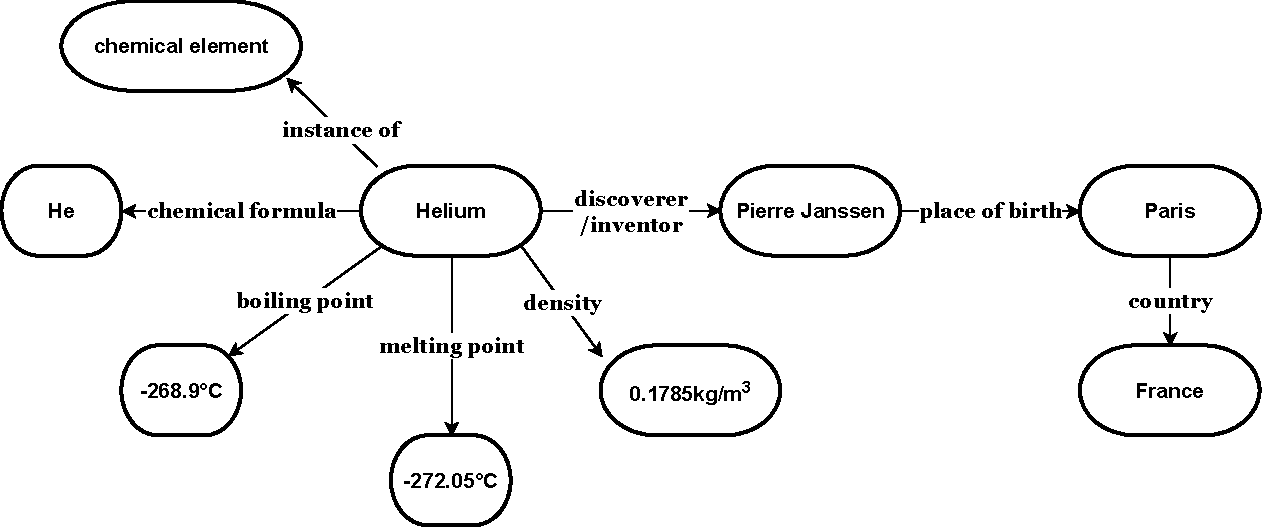
\includegraphics[width=0.80\linewidth]{images/del_graph.drawio.pdf}
  \caption{Directed edge-labelled graph describing Helium}
  \label{fig:figure 1}
\end{figure}

The technical of formal representation of graphs in RDF makes use of some important terms - IRIs, RDF literals and blank nodes. We discuss these briefly before giving a formal definition of RDF graphs.




\subsection*{IRI}
%\subsubsection{IRIs}

In order to exchange graphs across the web we need to identify resources uniquely. For this identification, we use identifiers in RDF called IRIs. 

A Uniform Resource Identifier (\acrshort{URI}) is a sequence of a subset of ASCII characters that identifies any web resource by using a name, a location, or both. They have a scheme, authority, path, and query and fragment, where all parts other than scheme and path are optional. URIs are of the form \textbf{scheme:[//authority]path[?query][\#fragment]}. For example, \textit{http://www.wikidata.org/entity/Q560} is an IRI that identifies the chemical element Helium on Wikidata. A Uniform Resource Locator (\acrshort{URL}) is a subset of URI that is used to specify the location of a digital document.

An Internationalized Resource Identifier (\acrshort{IRI}) is a generalized form of URI that helps to distinguish resources with Unicode. Basically, the character set in URI is extended to the Universal Coded Character Set. This enables it to contain any Latin and non-Latin characters except the reserved characters.

In RDF an IRI is used as a name (can be thought of as an ID) for graph nodes. It defines the resources that appears as nodes or edge labels in a RDF graph. There are already several pre-existing IRIs available for common use. New domain specific IRIs can be created based on the application. However, we must ensure there no conflicts with other IRIs available on the web.

\subsection*{RDF Literals}
%\subsubsection{RDF Literals}

We do not represent data values in RDF by IRIs. The data values do not need to be identified uniquely since they share the same meaning in every application. RDF data values or literals are used to represent resources that have values belonging to datatypes. Each literal can have only one datatype. RDF literals are written in the format "lexical value" \textasciicircum\ textasciicircum datatype-IRI, where lexical value is a string and datatype is an IRI. For example, the boiling point of helium is represented as -268.9^^xsd:decimal (footnote: abbreviation for 268.9^^http://www.w3.org/2001/XMLSchema\#decimal) in RDF. In RDF graphs, we use rectangular nodes for RDF literals.

The W3C standard XML Schema defines the datatypes and their IRIs. For example, decimals are identified by the IRI http://www.w3.org/2001/XMLSchema\#decimal. W3C has a good documentation on the different XML Schema built-in datatypes \cite{R.Cyganiak2014}. 

The datatypes in RDF are specified by three components – value space, lexical space and lexical-to-value mapping. The value space is the set of all possible values that a datatype can have. There are many datatypes in RDF such as string, Boolean, decimal and integer(footnote:A full list is available on the W3C’s section on RDF datatypes: www.w3.org/TR/2014/REC-rdf11-concepts-20140225/\#section-Datatypes). The lexical value is a string (footnote: RDF is based on Unicode strings) that corresponds to a particular literal value in the value space.

The lexical space contains a set of strings (footnote: RDF is based on Unicode strings) that are used to denote the values of the datatype. Lastly, the lexical-to-value mapping is a function that maps each string in the lexical space to an element in the value space. 

For instance, the datatype boolean has the set {true, false} in the value space and the set {true, false, 1, 0} in the lexical space. The strings true and 1 from the lexical space are mapped to true that belongs to the value space. Similarly, the strings false and 0 are mapped to 0. 

In RDF we can use a language-tagged string to denote a string in a specific language. This helps to provide human-readable labels to RDF literals. A literal is a language-tagged string is of the form "string"@language (footnote: Here language is a well-formed language tag (after BCP47). For example, the label for helium in French is hélium, and is denoted as "hélium"@fr in RDF. We normally ignore the datatype IRI (http://www.w3.org/1999/02/22-rdf-syntax-ns\#langString) when representing string literals. 


\subsection*{Blank Nodes}
%\subsubsection{Blank Nodes}
Blank nodes in RDF, also known as a bnode, do not identify specific resources as IRIs or literals do. They are used as placeholders for some nodes, i.e., to say that something exits at the position, without specifying what the node actually is. Fig XYZ shows the use of a blank node in RDF. The information for the address is of multi-component structure and we use a blank node in its place. The domain http://example.org is just an example domain and does not identify a real RDF data source.

\begin{figure}[h]
  \centering
  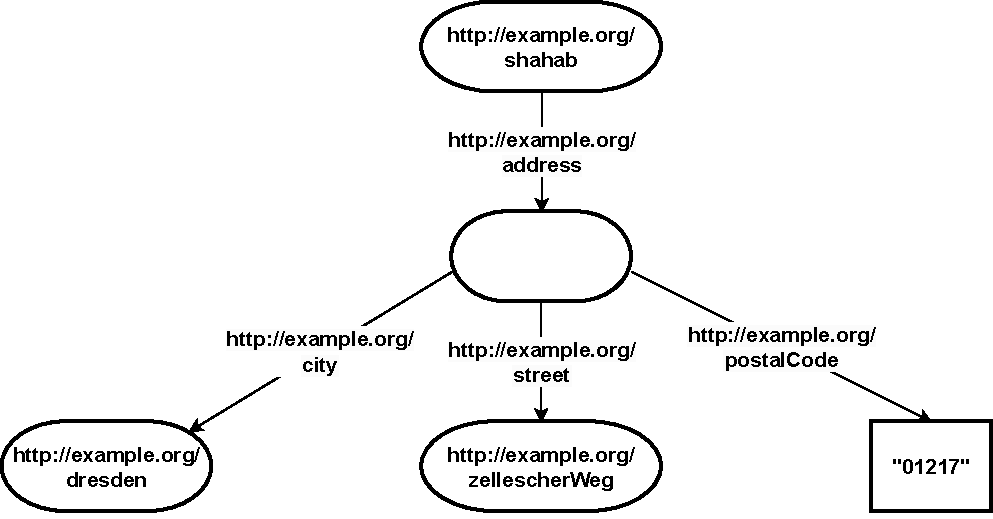
\includegraphics[width=0.80\linewidth]{images/blank_node.drawio.pdf}
  \caption{Directed edge-labelled graph describing Helium}
  \label{fig:figure 1}
\end{figure}

\subsection{RDF Graph}
\begin{definition}[RDF Graph]	
An RDF graph is a directed edge-labelled graph composed of a set of triples. A triple, also known as statement, represents the relationship between a subject and an object, linked by a predicate. The subject and object nodes are the source and destination nodes respectively. Formally, each triple consist of the following elements:   

\begin{itemize}
	\item a subject node that is an IRI or a blank node
	\item a predicate edge that is an IRI
	\item an object node that is an IRI, a blank node, or a literal
\end{itemize}	
\end{definition}

Figure XYZ shows RDF graph of our example represented in Fig 2. We use the http://www.w3.org/2000/01/rdf-schema\#label property in RDF to provide a human-readable version of a resource's name.

\begin{figure}[h]
  \centering
  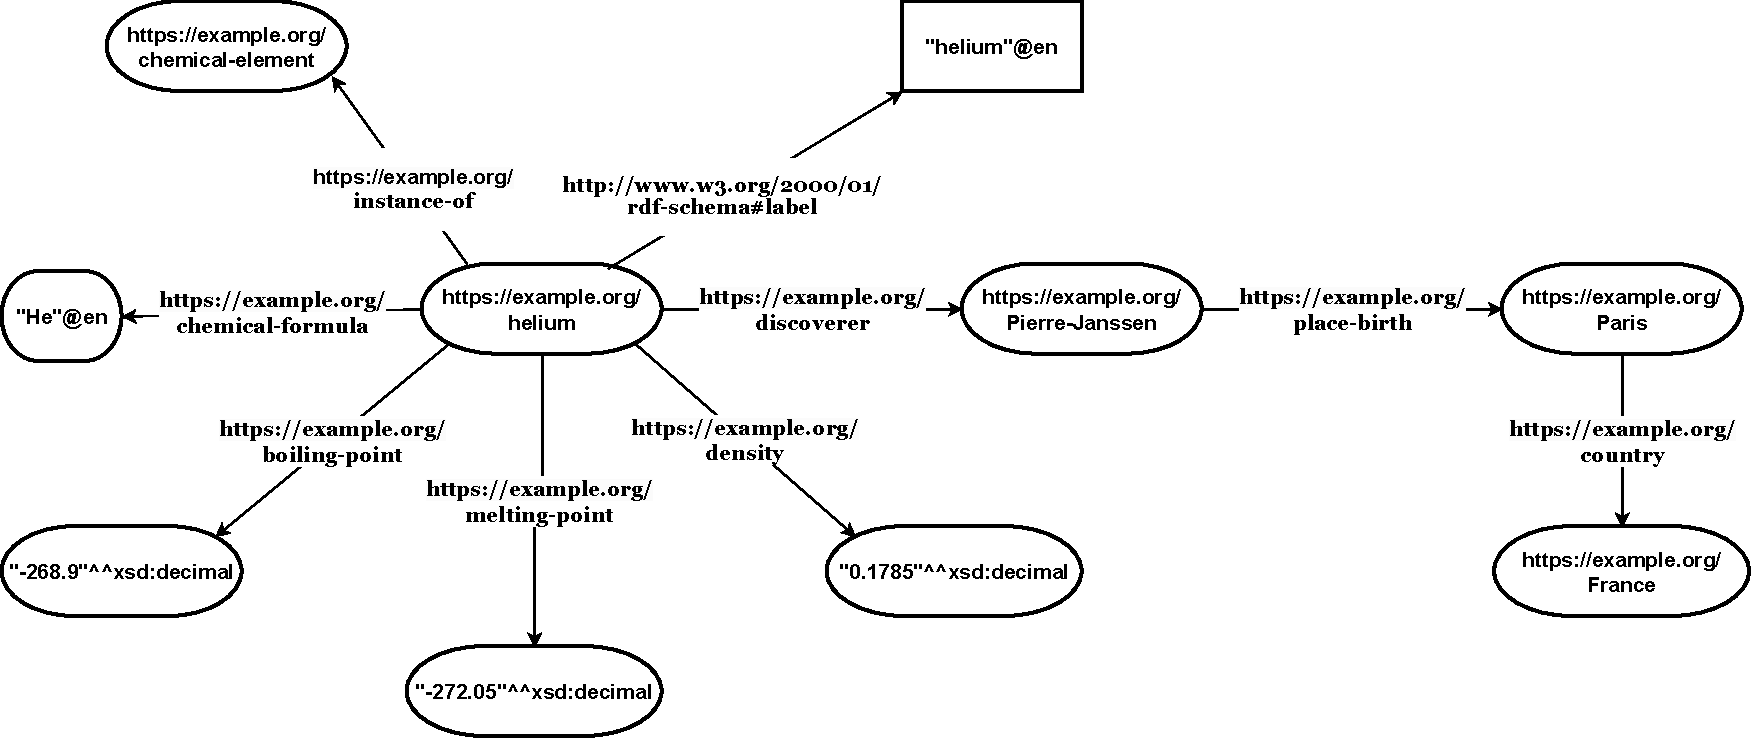
\includegraphics[width=0.75 \linewidth]{images/rdf_graph_updated.drawio.pdf}
  \caption{An RDF graph with Subject and Object nodes connected via a predicate edge}
  \label{fig:figure 2}
\end{figure}


In RDF, IRIs and literals denote resources, also called entities. In chapter 1, we defined entities to be real world objects and abstract concepts. The predicate edge is also denoted by an IRI and represents a property. In other words, it represents a binary relation between the entities. RDF defines some resources and properties using its vocabulary. An RDF vocabulary is a collection of IRIs that we can use in RDF graphs. The RDF vocabulary is defined in the namespace http://www.w3.org/1999/02/22-rdf-syntax-ns\#, normally prefixed as "rdf:". For example rdf:HTML and rdf:type are RDF voocabularies.

RDFS extends the RDF vocabulary and is defined in the namespace http://www.w3.org/2000/01/rdf-schema\#, prefixed normally as "rdfs:" such as rdfs:class and rdfs:label. It provides mechanisms that allow for the depiction of groups of interconnected resources and their interrelationships. Resources can be divided into groups known as classes, and classes themselves are also resources \cite{Brickley2014}. A resource belonging to a class is known to be an instance of that class. The property rdf:type is used to represent this via the statement "X rdf:type Y", denoting X to be an instance of Y. We can recall that an RDF triple is called a statement. For example, from the RDF graph in Fig XYZ we see that https://example.org./helium is an instance of the class https://example.org./chemical-element. 


%\begin{table}[b!]
%	\begin{center}
%		\caption{Abbreviation/IDs and their meanings.}
%		\label{tab: table 1}
%		\begin{tabular}{c|c}
%%			\textbf{Benchmarking tool} & \textbf{Resource monitoring tool} & \textbf{License} & \textbf{Updated} \\ \hline
%			wd & http://www.wikidata.org/entity/ \\ \hline
%			wdt & http://www.wikidata.org/prop/direct/ \\ \hline
%			rdfs & http://www.w3.org/2000/01/rdf-schema\# \\ \hline
%			Q560 & Helium \\ \hline
%			Q298581	& discoverer/inventor \\ \hline
%			Q90 & Paris \\ \hline
%			P31	& instance of \\ \hline
%			P274 & chemical formula \\ \hline
%			P2102 & boiling point \\ \hline
%			P2101 & melting point \\ \hline
%			P2054 & density \\ \hline
%			P61	& discoverer/inventor \\ \hline
%			P19	 & place of birth \\ \hline
%			P625 & coordinate location
%		\end{tabular}
%	\end{center}
%\end{table}


\subsection{Serialisations}
For exchanging graphs across the web, we need a syntactical representation of RDF. There are different formats available (footnote: A full list along with explanation is available on the W3C’s section on RDF Syntax https://www.w3.org/wiki/RdfSyntax), the most common ones are N-Triples, Turtle, JSON-LD, RDF/XML and RDFa. In this report, we focus on N-Triples and Turtle.

\subsubsection{N-Triples}
N-Triples represents RDF graphs in a simple line-based format.\footnote{Full specification available at: https://www.w3.org/TR/n-triples/ .} Every triple is encoded in a single line. The IRIs are written within pointy brackets and literals are written as lexical value\textasciicircum \textasciicircum datatype-IRI. Blank nodes are represented as \_:stringID, where stringID can be any string used to identify the blank node in the document. After every element of a triple there is a whitespace, and all the lines end with a dot. We can use comments using hash symbol after the end of every triple in a line or in a single dedicated line, and they are treated as white spaces. The files are saved with a \textit{.nt} extension.

Listing~\ref{listing:listing1} shows the representation of the RDF graph in Figure~\ref{fig:figure 3} in N-triples format. We have given line breaks for better readability.

\begin{minipage}{\linewidth}
\begin{lstlisting}[columns=fullflexible, label=listing:listing1, caption={RDF graph represented in N-triples syntax}, language=SPARQL]

<https://example.org/helium> < http://www.w3.org/2000/01/rdf-schema#type>
%\phantom{<http://www.wikidata.org/entity/Q560> <http://www.}%<https://example.org/chemical-element> .
		                                                
<https://example.org/helium> <http://www.w3.org/2000/01/rdf-schema#label> 
%\phantom{<http://www.wikidata.org/entity/Q560> <http://www.}%"helium"@en .

<https://example.org/helium> <https://example.org/chemical-formula> 
%\phantom{<http://www.wikidata.org/entity/Q560> <http://www.}%"He"@en .

<https://example.org/helium> <https://example.org/boiling-point> 
%\phantom{<http://www.wikidata.org/entity/Q560> <http://www.}%"-268.9"^^<http://www.w3.org/2001/XMLSchema#decimal> .

<https://example.org/helium> <https://example.org/melting-point> 
%\phantom{<http://www.wikidata.org/entity/Q560> <http://www.}%"-272.05"^^<http://www.w3.org/2001/XMLSchema#decimal> .

<https://example.org/helium> <https://example.org/density> 
%\phantom{<http://www.wikidata.org/entity/Q560> <http://www.}%"0.1785"^^<http://www.w3.org/2001/XMLSchema#decimal> .

<https://example.org/helium>  <https://example.org/discoverer> 
%\phantom{<http://www.wikidata.org/entity/Q560> <http://www.}%<https://example.org/Pierre-Janssen> .

<https://example.org/Pierre-Janssen> <https://example.org/place-birth> 
%\phantom{<http://www.wikidata.org/entity/Q560> <http://www.}%<https://example.org/Paris> .

<https://example.org/Paris> <https://example.org/country>
%\phantom{<http://www.wikidata.org/entity/Q560> <http://www.}%<https://example.org/France> .

\end{lstlisting}
\end{minipage}

\subsubsection{Turtle}
Turtle is an easy to read representation of RDF graphs. It extends the N-Triples format by providing several simplifications.\footnote{Full specification available at: https://www.w3.org/TR/turtle/ .} We can use prefix declarations and base namespaces at the beginning of the file to shorten IRIs. Turtle allows us to avoid repetition. We can use a semicolon at the end of a line instead of a dot if we know the next line has the same subject. Consequently, the next line will only have a predicate and object omitting the subject. Also, we can use a comma at the end of a line if we know the next line will start with the same subject and predicate. Analogously, the next line will only have a an object omitting the subject and the predicate. Blank nodes are represented using only square brackets. Additionally, we can provide predicate-object pairs within the square brackets to give further triples keeping the blank node as the subject. Turtle also provides a shorthand syntax for writing numbers. Numbers of the datatype integer, decimal and double can be written without quotes and datatype-IRIs. Boolean values can be written directly as either "\textit{true}" or "\textit{false}". The files are saved with a \textit{.ttl} extension.

Listing~\ref{listing:listing2} shows the representation of the RDF graph in Figure~\ref{fig:figure 3} in Turtle format. 

\begin{minipage}{\linewidth}
\begin{lstlisting}[label=listing:listing2, caption={RDF graph represented in Turtle syntax}, language=SPARQL]

BASE <https://example.org/>
PREFIX rdfs: <http://www.w3.org/2000/01/rdf-schema#>
PREFIX rdf: http://www.w3.org/2000/01/rdf-schema#
PREFIX xsd: <http://www.w3.org/2001/XMLSchema#>

<helium> rdf:type <chemical-element> ;
%\phantom{wd:Q560 }% rdfs:label "helium"@en ;
%\phantom{wd:Q560 }% <chemical-formula> "He"@en ;
%\phantom{wd:Q560 }% <boiling-point> -268.9 ;
%\phantom{wd:Q560 }% <meling-point> -272.05 ;
%\phantom{wd:Q560 }% <density> 0.1785 ;
%\phantom{wd:Q560 }% <discoverer> <Pierre-Janssen> .
<Pierre-Janssen> <place-birth> <Paris> .
<Paris> <country> <France> .
\end{lstlisting}
\end{minipage}



\section{Wikidata}
%\subsection{Wikidata}

Wikidata is built on the RDF framework. However, it does not define its resources in terms of RDFS. Instead, it has its own data model known as Wikibase data model (footnote: https://www.mediawiki.org/wiki/Wikibase/DataModel). This data model can be expressed in RDF but there are some important differences compared to the standard Linked Data practices that RDF follows. 

Wikidata defines its own classes and properties that are equivalent to RDF constructs. For example, to denote that the subject is an instance of a class, Wikidata uses the instance of property instead of the rdf:type property in RDF. Wikidata offers an explanation for some of the standards properties in Wikidata that correspond to the ones in RDF \cite{Foundation}. 

Unlike RDF, statements in Wikidata are ranked. Additionally, they can have annotations and references. In Section XYZ we discussed that data types in RDF are mapped to XML Schema data types. However, property types in Wikidata are not defined in terms of XML Schema types. They are defined in terms of the types of values that the properties can have. For example, the "element symbol" property in Wikidata (\footnote: https://www.wikidata.org/wiki/Property:P246) has the property type of "String" indicating it can gave values that are strings.

Resources in Wikidata are called entities, and each entity is uniquely identified by an entity ID. The next section describes Wikidata entities and statements in detail.


\subsection{Entities}
Wikidata maintains its data structure by pages. Each entity has a dedicated page for itself and is identified by an unique ID.  Basically, every element on which Wikidata has structured data is known as an entity\cite{Erxleben2014}. Entities are identified by an unique ID and not by names or labels. Wikidata has mainly three types of entities – items, properties and lexemes. Other extensions can define new entity types such as MediaInfo and subentities like Form and Sense. We refer to items and properties when mentioning entities. The rest are out of the scope of this report.

Items are real-world objects, concepts or events.  These generally have a page in Wikipedia. For instance, there is an English Wikipedia on Helium (footnote: https://en.wikipedia.org/wiki/Helium). Here the item is Helium and Wikidata records facts about it. (footnote: https://www.wikidata.org/wiki/Q560.) Each item is identified by a QID - an ID prefixed with the letter "Q" followed by a number. For example, the item helium has the QID of Q560. Items in Wikidata belong to the main namespace - http://www.wikidata.org/wiki/QID. 

Properties describe the relationship between entities and property values. Each property in Wikidata has a datatype that specifies the type and shape of the values assigned to the property. In other words, datatypes determine which values the property can accept, such as string, quantity or time. (footnote: Wikidata provides a list of all the datatypes: https://www.wikidata.org/wiki/Special:ListDatatypes.). Properties are identified by a PID - an ID prefixed with the letter "P" and followed a number. They belong to the property namespace in Wikidata - http://www.wikidata.org/wiki/Property:PID. 

Every entity constitutes of the following main parts - labels, descriptions, aliases, and statements. Items also have sitelinks. Labels, descriptions and aliases are multilingual which help to find the respective entity. They are used to identify them clearly, since entities are identified by IDs and are not understood by humans. Sitelinks provide links about an individual item to external pages on other Wikimedia sites such as Wikipedia. 

A statement in Wikidata consists of a claim and references. Claims are property-value pairs, which along with the entity form a RDF triple, where the entity is the subject. Claims can also contain optional qualifiers that provide some additional information for the claim. This information is in the form of property-value pairs that refer to the claim instead of the entity. References point to specific resources that support the claim of statement. They can be links to URLs or items.

An entity can have several statements for the same property, and all of them might not necessarily be important or relevant. Ranks are used as a quality factor to distinguish between several statements. A Wikidata statement can have one of three types of ranks - "normal", "preferred" and "deprecated". By default, a statement has the normal rank unless changed to preferred or deprecated. A statement with preferred rank means it should be given priority over the normal ranked statements. A deprecated rank indicates that the statement is incorrect or under discussion, and it may have a reference. Deprecated statements are kept either for the sake for completion or to prevent users from constantly adding or removing them. Wikidata has around 100 million items (footnote: https://grafana.wikimedia.org/d/000000167/wikidata-datamodel) and around 1.43 billion item statements as of December 2022 (footnote: https://grafana.wikimedia.org/d/000000175/wikidata-datamodel-statements). 

Figure 4 shows an excerpt of the Wikidata page on the item Helium (footnote: https://www.wikidata.org/wiki/Q560). We can see Helium has the QID of Q560, and has labels, descriptions and aliases in different languages. It has a sitelink for the item in Wikipedia offered in 186 languages. We show one of the statements that has a claim indictaing that Helium has the instance of property with chemical element as the value. The property-value pairs follows, hydrogen and followed by, lithium are qualifiers of the claim. At the time of this writing, there are no references provided for this claim. This statement hence gives us the information that Helium is an instance of chemical element, and it comes after the element hydrogen and if followed by the element lithium. The statement has has the normal rank (indicated by the middle portion greyed). 

Figure 5 shows an excerpt of the property instance of page on Wikidata (footnote: https://www.wikidata.org/wiki/Property:P31). The property has a PID of P31 along and with multilingual labels, descriptions and aliases. The statement has a claim indicating that this property also has an instance of property with Wikidata property being the value. The claim has no qualifiers and there are no references to support it. The instance of property accepts the datatype item as a value. The rank for this statement is normal.

\begin{figure}[h]
  \centering
  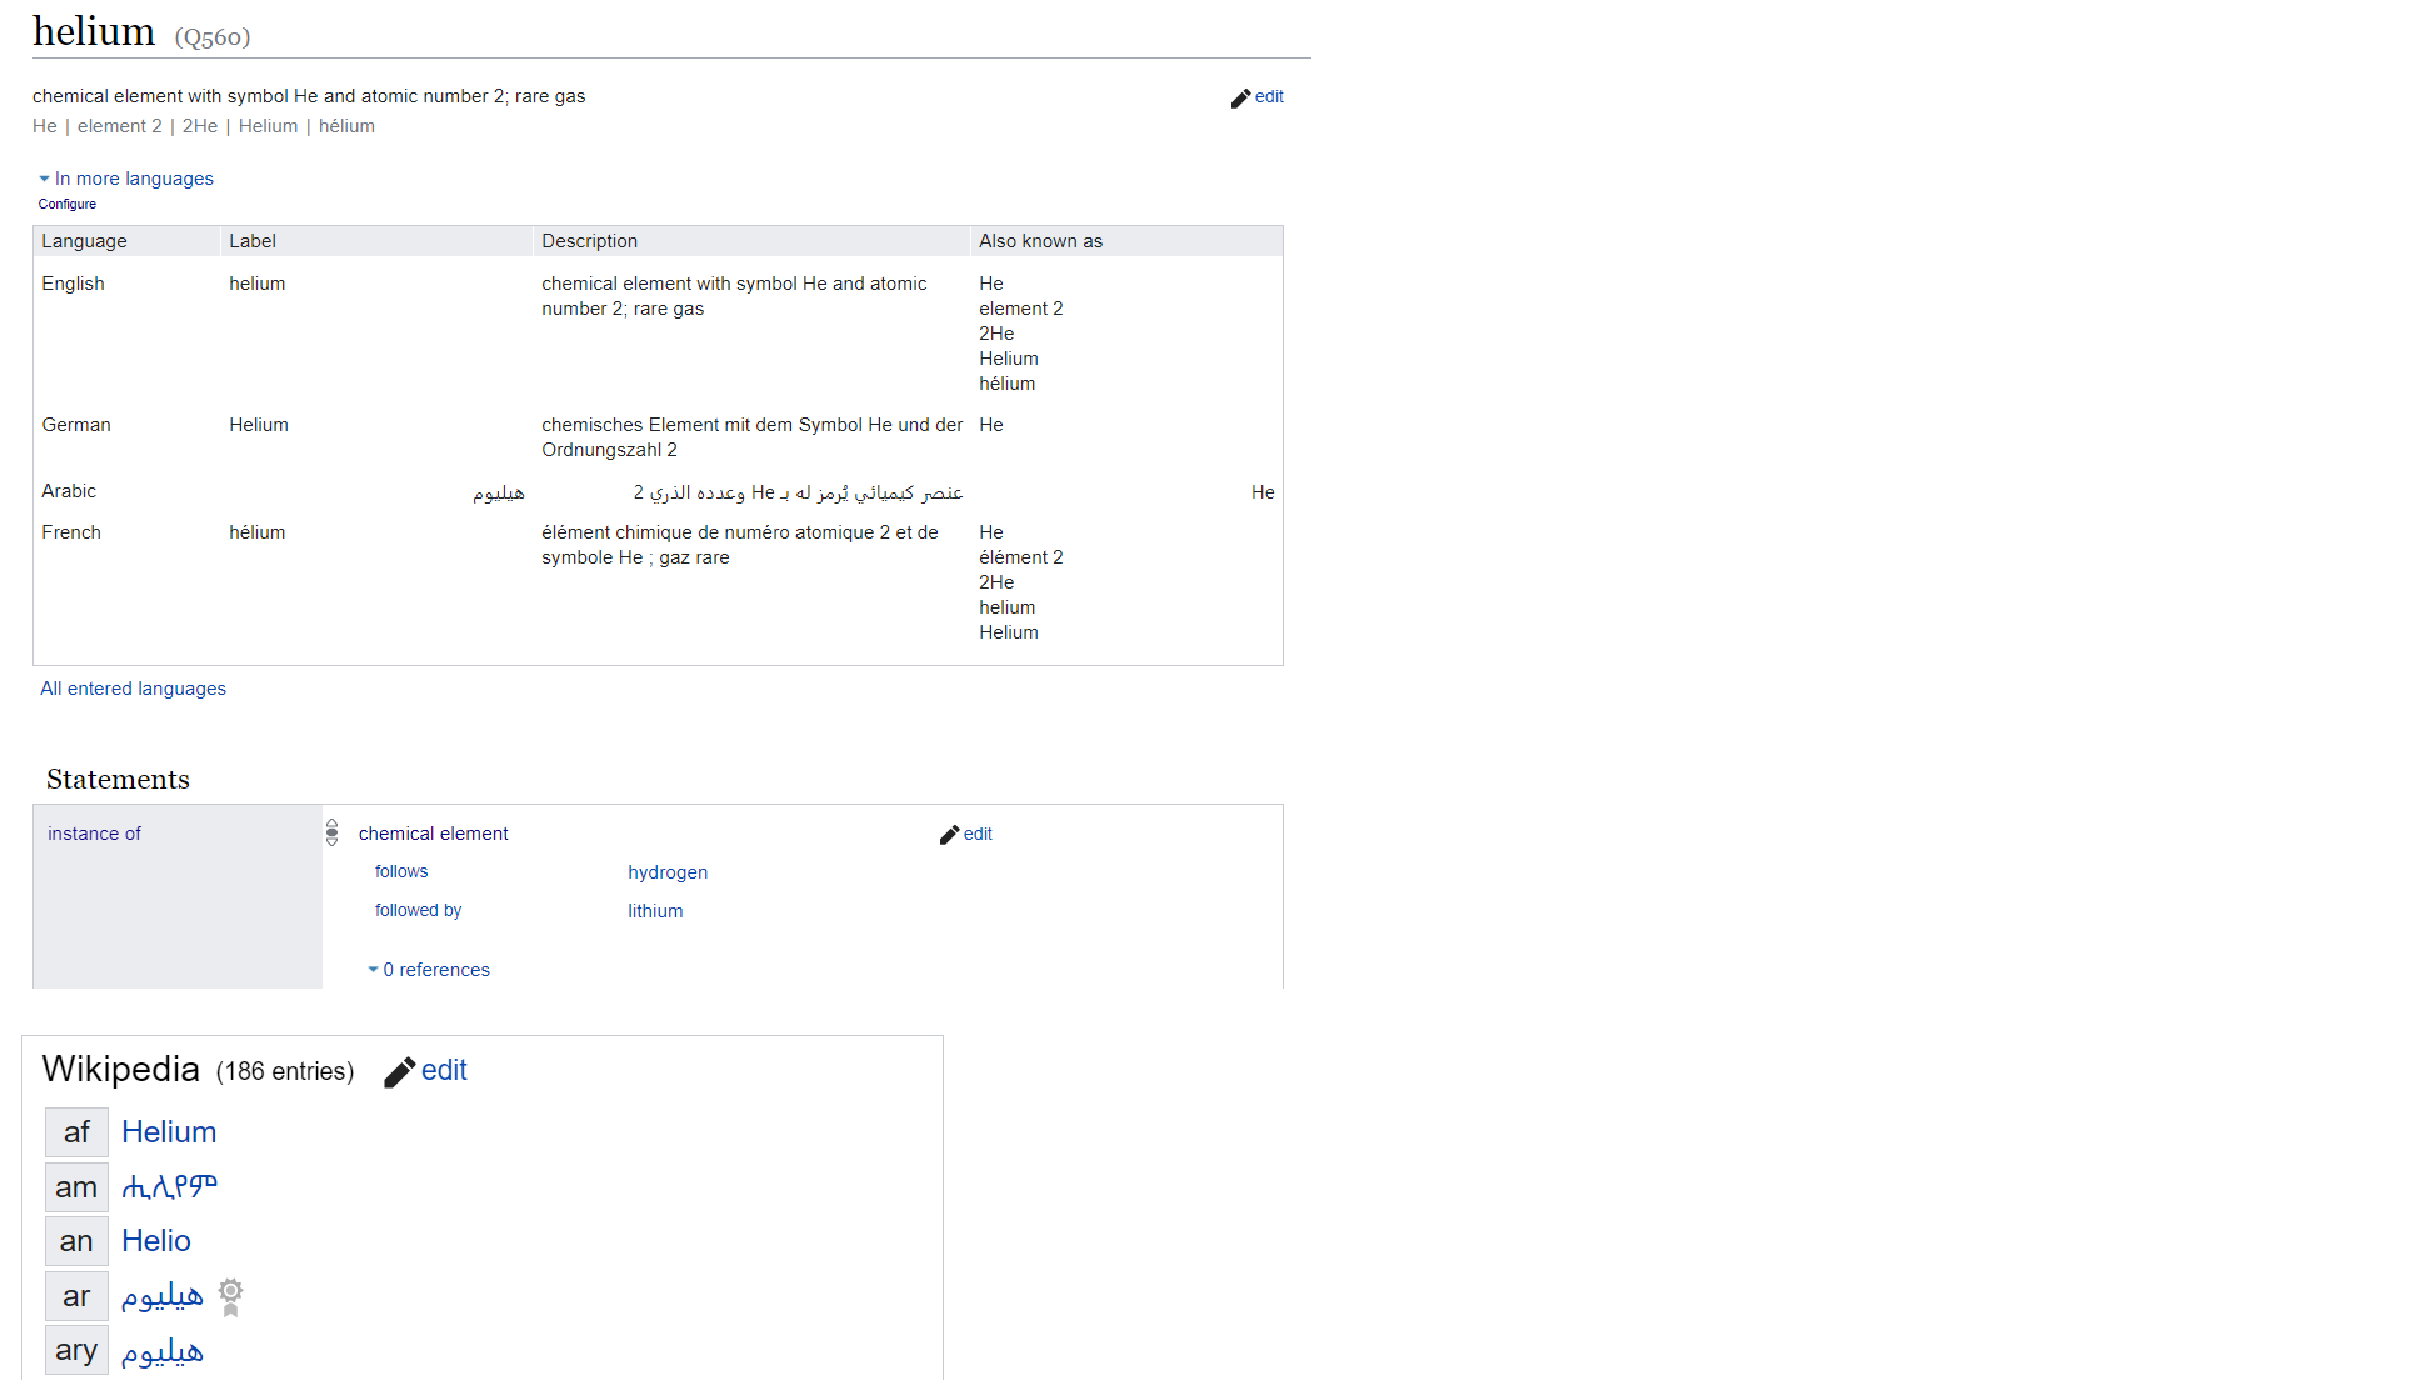
\includegraphics[width=0.75 \linewidth]{images/helium.pdf}
  \caption{RDF graph describing Helium}
  \label{fig:figure 3}
\end{figure}

\begin{figure}[h]
  \centering
  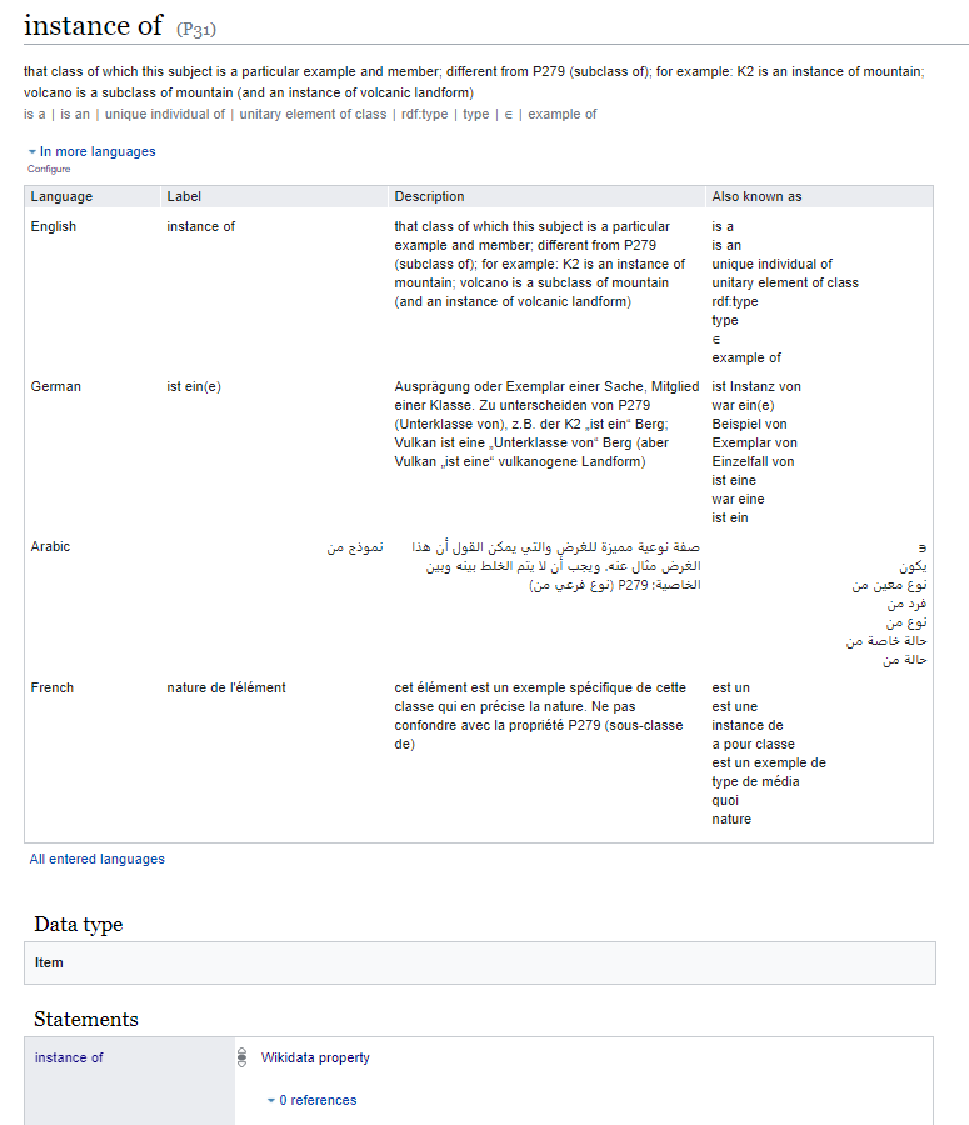
\includegraphics[width=0.75 \linewidth]{images/instance_of.pdf}
  \caption{RDF graph describing Helium}
  \label{fig:figure 3}
\end{figure}


The RDF graph in Fig XYZ used the example.org domain and the resources identified with this domain do not point to any real data about helium. Fig XYZ show information about helium taken from Wikidata. 


\begin{figure}[h]
  \centering
  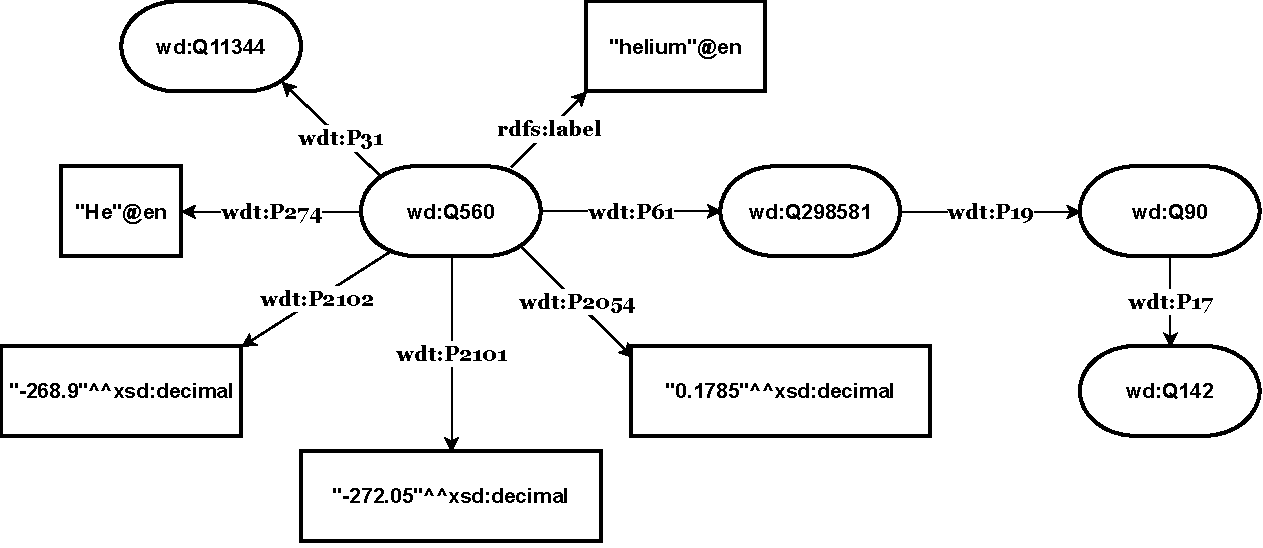
\includegraphics[width=0.75 \linewidth]{images/wikidata_graph.drawio.pdf}
  \caption{RDF graph describing Helium}
  \label{fig:figure 3}
\end{figure}

Entity nodes are represented using wd: (footnote: http://www.wikidata.org/entity/) followed by the QID for items and PID for properties. In our example, we represent only truthy statements. This refers to statements that have the best non-depreciated rank for a given property. This refers to statements that hold the highest rank for a given property. If any statement has a preferred rank then that statement is considered truthy, otherwise the normal are ranked statements are considered truthy. Predicates for truthy statements are represented by wdt: (footnote: http://www.wikidata.org/prop/direct/) followed by the PID of the property. 


From Figure~\ref{fig:figure 3} we understand that \textit{Helium} \texttt{(\gls{Q560})} is an \textit{instance of} \texttt{(P31)} of \textit{chemical element} \texttt{(Q11344)}. It has a human understandable english \textit{label} called \textit{helium} and the \textit{chemical formula} \texttt{(P274)} of \textit{He}. Its \textit{boiling point} \texttt{(P2102)}, \textit{melting point} \texttt{(P2102)} and \textit{density} \texttt{(P2054)} are \textit{-268.9~°C}, \textit{0.1785~°C} and \textit{-272-05~kg/m3} respectively. Helium has a \textit{discoverer/inventor} \texttt{(P61)} by the name of \textit{Pierre Janssen} \texttt{(Q298581)}. His \textit{place of birth} \texttt{(P19)} was \textit{Paris} \texttt{(Q90)} that belongs to the \textit{country} \texttt{(P17)} of \textit{France} \texttt{(Q142)}.

\subsection{Querying Wikidata}

The easiest and most popular way to query Wikidata is through the Wikidata Query Service (WDQS). This is Wikidata's SPARQL endpoint. We can use this service two ways. Firstly, we can write queries in SPARQL directly on the web user interface of the service\footnote{https://query.wikidata.org/ .} and obtain the results in different formats like table, tree, graph, etc. Secondly, the service can also be used progmatically by submitting GET or POST requests.\footnote{https://query.wikidata.org/sparql.}

Another popular way to query Wikidata is by using the Wikidata API.\footnote{https://www.wikidata.org/wiki/Special:ApiSandbox.} However, this API should mainly be used when we want to edit the contents of Wikidata or get data about entities like revision history.

Wikidata dumps is useful when we know our result set will be significantly large or if we want to set up our own local query service. These dumps are full exports of all the available entities in Wikidata.\footnote{https://dumps.wikimedia.org/ .} To get started you should download the latest complete dump.\footnote{https://dumps.wikimedia.org/wikidatawiki/latest/ .} Wikidata also mentions some other ways to accessing Wikidata's data like Search and Linked Data Fragments endpoint, the complete list and usage of which can be found on Wikidata's Data Access webpage \cite{ Wikidata2022}.




\section{SPARQL}
%\subsection{SPARQL}
SPARQL Protocol and RDF Query Language (SPARQL)\footnote{ https://www.w3.org/TR/sparql11-overview/} is a W3C recommended query language for RDF. This means it allows to query any data source that can be mapped to RDF. It is also a HTTP-based protocol for linked open data on the web. This enables the transmission of SPARQL queries and results between a client and a SPARQL engine. The first working draft for SPARQL was released in 2004 and it became a W3C Recommendation in 2008 \cite{Perez2009}. 

Queries in SPARQL are based on matching graph patterns and can be used to retrieve, add or delete data in the RDF based dataset. In section XYZ we saw that RDF data is based on triples - subject, object and predicate. Consequently, a query in SPARQL consists of a set of triple patterns. Each of the elements of the triple can be a variable (a string beginning with ? or \$) that needs to be queried. The solution to the variables is obtained by matching the query patterns to the triples in the dataset.

There are four forms of queries - SELECT, ASK, CONSTRUCT and DESCRIBE. 
\begin{itemize}
\item SELECT queries select some or all the pattern matches and provides the results in a tabular format
\item ASK queries check whether there is at least one match and the result is true or false
\item CONSTRUCT queries create an RDF graph based on the query results
\item DESCRIBE queries return a RDF graph providing additional information on each results
\end{itemize}

In our work, we only consider SELECT queries. These consist of the following major blocks:
\begin{itemize}
\item Prologue: PREFIX and BASE keywords that function similarly to those in RDF turtle format
\item Select clause: SELECT keyword followed by either a list of variables and variable assignments, or by *
\item Where clause: WHERE keyword followed by a query graph pattern to be matched
\item Solution set modifiers: Change the set of solutions using modifiers such as LIMIT and OFFSET
\end{itemize}

The select and where clauses are mandatory, the rest being optional. Other optional features are filters, groups, query operators such as UNION, OPTIONAL and BIND, and aggregates. A full specification for the query language can be found on the official W3C documentation\cite{Seaborn}.

Listing~\ref{listing:listing3} shows an example of querying Wikidata using SPARQL. We want to get a a list of all chemical elements, along with their English labels, that have a chemical formula, boiling point, melting point, density, an inventor/discoverer, birth place of that inventor/discoverer and the country that the place belongs to. Since there might be several results, we are limiting them to five using the LIMIT keyword. The namespace http://www.wikidata.org/entity/ is used for items when querying. We are interested in the truthy values of the properties and so the namespace http://www.wikidata.org/prop/direct/ is used for properties. Truthy values are essentially the values for which the statement has the best non-deprecated rank. This means that if a statement has preferred rank then that statement is considered to be truthy. Otherwise, the normal ranked statement is taken to be truthy. The PREFIX is optional since Wikidata recognizes the short forms wd and wdt automatically. Turtle syntax that we saw in section XYZ can be applied in SPARQL. The query can be run in Wikidata's query service.\footnote{https://query.wikidata.org/ .}  

\begin{minipage}{\linewidth}
\begin{lstlisting}[label=listing:listing3, caption={Querying Wikidata with SPARQL}, language=SPARQL]

PREFIX wd: <http://www.wikidata.org/entity/>
PREFIX wdt: <http://www.wikidata.org/prop/direct/>
SELECT *
WHERE {
  ?element wdt:P31 wd:Q11344 ;
  %\phantom{?element }% wdt:P274 ?element_formula ; 
  %\phantom{?element }% wdt:P2102 ?boiling_point ;
  %\phantom{?element }% wdt:P2101 ?melting_point ;
  %\phantom{?element }% wdt:P2054 ?density ;
  %\phantom{?element }% wdt:P61 ?discoverer .
  ?discoverer wdt:P19 ?place_birth .
  ?place_birth wdt:P17 ?country .
  FILTER(LANG(?element_label)="en")
}LIMIT 5

\end{lstlisting}
\end{minipage}

Table 1 shows the results obtained in a tabular form. Among the results, there is the element Helium (Q560) that we have used as an example in Fig 1 and Fig 3. 

\begin{table}[h]
	\begin{center}
		\caption{Results of the SPARQL query in Listing 2}
		\label{tab: table 1}
		\begin{tabular}{ccccccccc}
		
%		\textbf{element} & \textbf{element_formula} & \textbf{element_label} & \textbf{boiling_point} & \textbf{melting_point} & \textbf{density} & \textbf{discoverer} & \textbf{place_birth} & \textbf{country} \\ \hline
			\toprule
			
			\textbf{element} & \textbf{element\textunderscore formula} & \textbf{element\textunderscore label} & \textbf{boiling\textunderscore point} & \textbf{melting\textunderscore point} & \textbf{density} & \textbf{discoverer} & \textbf{place\textunderscore birth} & \textbf{country} \\ 
		
			\midrule
			
			wd:Q560 & He & helium	& -268.9 & -272.05 & 0.1785 & wd:Q298581 & wd:Q90 & wd:Q142 \\
			
			wd:Q560 & He & helium & -268.9 & -272.05 & 0.1785 & wd:Q950726 & wd:Q4093 & wd:Q145 \\ 
			
			wd:Q560 & He & helium & -268.9 & -272.05 & 0.1785	 & wd:Q127959 & wd:Q623765 & wd:Q145 \\ 
			
			wd:Q670 & Si & silicon & 4271 & 2570	& 2.329	& wd:Q151911 & wd:Q1451001 & wd:Q34 \\ 
			
			wd:Q568	& Li & lithium	& 1317	& 180.5	& 0.535	& wd:Q313568 & wd:Q10495519 & wd:Q34 \\
			
			\bottomrule

		\end{tabular}
	\end{center}
\end{table}

\section{GraphQL}
GraphQL (Graph Query Language) is an open source query language for APIs (Application Programming Interfaces) and a server-side runtime for executing queries. It is data source agnostic, i.e., it is not tied to any particular data source such as a database. The data could be stored in different sources such as databases or micro-services.

With a single API call, GraphQL can aggregate data from multiple sources and resolve the data to the client. This is one of the advantages GraphQL has over REST API where the latter would require several HTTP calls to access data from multiple sources. 

GraphQL is also language agnostic. This means that GraphQL services, such as the schema and resolvers, can be written in any programming language such as JavaScript or Python. GraphQL API is usually served over HTTP through a GraphQL server. A GraphQL server consists of two main parts – schema and resolver. 

The schema defines object types that have fields. The object types represent the kind of objects that can be fetched from the data source. The fields have values that can be other object types or scalar types such as Int or String. (footnote: GraphQL defines some default scalar types: https://graphql.org/learn/schema/\#scalar-types.) The purpose of the fields is to define the relationships between the object type and other types. This can be modelled as a directed graph where types are the nodes and fields are the edges. 

When a client sends a query request to the GraphQL server, it is parsed and the operation type is identified. The server then validates the request by checking it against the defined schema. If it fails then an error is returned otherwise the operation is executed and the resolvers process and retrieving values from the data source.

For the sake of human readability, GraphQL specification has its own Schema Definition Language (SDL). It is simple to write and understand schemas in SDL, and is similar to the language that we use to write queries. Listing XYZ shows a schema written in SDL. This schema can be in the GraphQL server against which clients can send queries for instances of chemical elements that have a name, chemical formula and boiling point. The exclamation mark means that the corresponding field is non-nullable and it is expected that GraphQL will give a value when the field is queried. A complete guide on schemas and types can be found on the official documentation from GraphQL (footnote: https://graphql.org/learn/schema/). 


\begin{minipage}{\linewidth}
\begin{lstlisting}{gql.py:GraphqlLexer -x}[label=listing:listing4, caption={Schema used to query a chemical element}]
type ChemicalElement{
	name: String!
	chemicalFormula: String!
	boilingPoint: Float!
}

\end{lstlisting}
\end{minipage}

A resolver in GraphQL server is a function that is associated with every field. It contains instructions on how to process that particular field. In other words, the resolver is responsible for retrieving a value from the data source.
 
A GraphQL query has a tree-like structure. The root node is at the top level and represents the parent node or objects. The leaf nodes represent the children nodes. To traverse the query we can follow this tree structure, i.e., we can go up to a parent node, down to a child node or left/right to a sibling node \cite{Perez2009}. When querying the idea is to request for some fields on objects.

There are three operations types in GraphQL – query, mutation and subscription. Query operations are used to fetch or read data from a data source. They are similar to GET requests in REST (Representational State Transfer). Mutation operations allow modifying data on the source by updating, adding or deleting. Subscription operations notify us about some events related to the data in a source such as addition of new data.

Listing XYZ shows a GraphQL query that can be used complemented by the schema in Listing XYZ . It fetches the name, chemicalFormula and boilingPoint of Helium, where Helium is of type chemialElement. Running the query against some data source provides a sample result as shown in Listing XYZ. The results obtained are in JSON format. We see that the shape of the results is similar to the shape of our query. This is crucial to GraphQL as we always get the type of response we expect when we write queries. Defining the types and fields in the schema allows the server to know the fields that the client can query for an object type. Also, GraphQL ensures the queries to return predictable results by providing the clients with control over the content of the data they receive. Hence, there is not over or under fetching of data.

In GraphQL clients can fetch related data (fields in the query) with a single HTTP request made to the GraphQL server. This reduces network overheads and improves performance.



\begin{minipage}{\linewidth}
\begin{lstlisting}[label=listing:listing5, caption={Query to fetch chemical elements and their properties}]
query QueryChemicalElement (limit 2){
    chemicalElement{
		name
		chemicalFormula
		boilingPoint
	}
}
\end{lstlisting}
\end{minipage}

\begin{minipage}{\linewidth}
\begin{lstlisting}[label=listing:listing5, caption={Query to fetch chemical elements and their properties}]
{
	"data":{
		"chemicalElement":{
			"name": "helium",
			"chemicalFormula": "He",
			"boilingPoint": -268.9
		},
		{	
			"name": "silicon",
			"chemicalFormula": "Si",
			"boilingPoint": 4271
		}
	}
}

\end{lstlisting}
\end{minipage}

\anas{Lukas told to provide one example showing all imp features of GraphQL}

\anas{maybe change the list to a table}

GraphQL offers several features that enhance its functionality to fetch data. Some important ones are summarized below: (footnote: full list can be found at : https://graphql.org/learn/)

\begin{itemize}
\item Arguments – Objects and fields can have arguments passed as parameters

\item Aliases – The results of a field can be renamed to avoid any conflicts that might occur when querying for the same fields but with different arguments. 

\item Fragments – Reusable units for sets of fields to help avoid repetitions.

\item Operation name – We can set a name to our operation to help in debugging. The name must be preceded by the operation type. When no name is mentioned (as our example in Listing XYZ) the query operation is considered to be of type query 

\item Variables – Set arguments to fields dynamically

\item Directives – Used to modify the behavior of a field or fragment. There are two directives that must be supported by GraphQL servers: 

\begin{itemize}
\item @include(if: Boolean) -  Include the field in the result if the argument is true.
\item @skip(if: Boolean) -  Skip the field if the argument is true.
\end{itemize}

\item Mutations – Allow to modify data

\item Inline Fragments – Used to return an interface or a union type

\item Meta fields – The \_\_typename meta field can be used to get the name of the object type defined in the schema


\item Non-null – Can be used in queries and schemas to indicate that an argument or field cannot be null; specified by an exclamation mark 


\item Interfaces – An abstract type containing a set of fields. Object types must include these fields when implementing the interface.


\item Union types – Used to define a type that can represent several different types.

\item Pagination – Used to control the number of results returned and the offset of the first results. 

\item Introspection  - Query schema to find out the types, fields and directives defined in the schema
\end{itemize}

\section{GraphQL vs SPARQL}

GraphQL and SPARQL are query languages developed with different goals in mind. GraphQL is designed to provide an efficient and flexible way to fetch data from APIs. It solves issues that are typical with using REST APIs such as over or under fetching of data, and requiring multiple HTTPS requests to query related data. 

On the other hand, SPARQL is a query language and protocol developed for working with RDF data. It provides a standard and flexible way for querying data stored in RDF format. The data can be distributed over multiple sources. Since it is also a protocol, it allows interacting with RDF data over HTTP. 

SPARQL is immensely popular in the field of research and academia where it sued for querying and analysing. However, it has not seen much growth in commercial applications. GraphQL, on the other hand, is more popular among software and web developers. There are some valid reasons for this.  

Firstly, many developers are still not familiar witFh the Linked Data model of RDF and SPARQL. They are more used to working with technologies such as GraphQL and RESTAPIs. Secondly, GraphQL is simple to learn and work with since it has human-oriented syntax. Among other things, this benefits application development. SPARQL however, proves to be more complex. It has more syntactic verbosity owing to the descriptive nature of writing queries. The produced output from SPARQL queries contains a lot of unnecessary metadata that is not useful for web developers and need to be further parsed for using in web applications \cite{Lisena2018}. 

Moreover, retrieval of data from knowledge graphs using SPARQL is time consuming and proves to be a steep learning curve, the reason being that there is limited documentation available for proper ontology descriptions and examples of using queries for SPARQL endpoints \cite{Angele2022}. One of the other reasons for using GraphQL over SPARQL is that developers are more equipped in using nested objects that GraphQL offers \cite{Taelman2018}. They lack the experience to work with triples which is the main foundation of SPARQL. Moreover, fewer supporting tools and libraries exist for working and developing with SPARQL than with GraphQL \cite{Taelman2018}. As a result, developers working with SPARQL may need to write more custom code as opposed to when working with GraphQL APIs.

On the other hand, SPARQL also has some advantages over GraphQL. SPARQL queries represent full graphs while those of GraphQL represent trees \cite{Taelman2018}. This make SPARQL more expressive. RDF provides a system to build detailed structures from the meaning of data, and is hence more complete and capable than GraphQL schemas \cite{Dresslar2019}. Since SPARQL works with the schema organization of RDF, this makes it more powerful than GraphQL. With SPARQL we can write complex queries that can be used to retrieve or modify data \cite{Angele2022}. As a result it is capable to satisfy many complex use cases.

Also since GraphQL alone has no notion of semantics \cite{Taelman2018}, a schema needs to be defined by the GraphQL API developers for every interface they want the client to query. This makes it difficult to integrate data returned when querying multiple different sources. SPARQL however supports federated queries which makes it more powerful and rich. Lastly, when using GraphQL we cannot uniquely identify resources on the web but which is possible using URIs with SPARQL. In other words, GraphQL has no notion of global identifiers \cite{Taelman2018}.



\textcolor{red}{Talk also about differences in terms of complexity and expressivity}
